\documentclass[10pt,conference,a4paper]{IEEEtran}
\IEEEoverridecommandlockouts

\usepackage{cite}
\usepackage{amsmath,amssymb,amsfonts}
\usepackage{graphicx}
\usepackage{booktabs}
\usepackage{url}
\usepackage{xcolor}

% Fill-ins computed by research/experiments/iecbes_fillins.py
% (subject-cluster bootstrap B=2000, Holm m=8, TOST delta=0.02).

\begin{document}

\title{X-Step: Sparse Four-Site Plantar-Pressure Sensing\\
for Continuous Biomechanical Risk Monitoring}
\author{
\makebox[\textwidth][c]{%
  \parbox[t]{0.31\textwidth}{\centering
    Arjun Subramanian\\
    \scriptsize
    \textit{Computer Science and Artificial Intelligence Lab (CSAIL)}\\
    \textit{Massachusetts Institute of Technology (MIT)}\\
    Cambridge, MA, USA\\
    arjun\_s@mit.edu
  }%
  \hspace{0.02\textwidth}%
  \parbox[t]{0.31\textwidth}{\centering
    Deeptanshu Devatha\\
    \scriptsize
    \textit{Artificial Intelligence, Explainability, and Accountability (AIEA) Lab}\\
    University of California, Santa Cruz\\
    Santa Cruz, CA, USA
  }%
  \hspace{0.02\textwidth}%
  \parbox[t]{0.31\textwidth}{\centering
    Hrudhai Lothumalla\\
    \scriptsize
    \textit{Artificial Intelligence, Explainability, and Accountability (AIEA) Lab}\\
    University of California, Santa Cruz\\
    Santa Cruz, CA, USA
  }%
}\\[1.5em]
\makebox[\textwidth][c]{%
  \parbox[t]{0.31\textwidth}{\centering
    Arnav Katelwale\\
    \scriptsize
    \textit{Artificial Intelligence, Explainability, and Accountability (AIEA) Lab}\\
    University of California, Santa Cruz\\
    Santa Cruz, CA, USA
  }%
  \hspace{0.02\textwidth}%
  \parbox[t]{0.31\textwidth}{\centering
    Leilani Gilpin\\
    \scriptsize
    \textit{Artificial Intelligence, Explainability, and Accountability (AIEA) Lab}\\
    University of California, Santa Cruz\\
    Santa Cruz, CA, USA\\
    lgilpin@ucsc.edu
  }%
}%
}
\maketitle

\begin{abstract}
Repetitive plantar overload is a mechanical ingredient of diabetes-related
foot disease, yet dense in-shoe arrays remain costly and largely
laboratory-bound. Sparse insoles are cheap enough for unsupervised wear, but
three questions are rarely answered together: how much label information four
sites actually retain, what subject-independent evaluation costs, and how the
pipeline fails under wearable faults. We specify X-Step---force-sensitive
resistors at MET1, MET2, MET5 and the heel, sampled at 25\,Hz on an ESP32 and
streamed as a documented 28-byte Bluetooth Low Energy frame---and analyse it
under an explicit measurement model with pre-specified estimands on a synthetic
24-subject, 2592-window cohort. Logistic regression reached macro-F1 0.885
(0.873--0.894) against 0.040 for a majority baseline, while independent-window
splitting reached 0.931, so the 0.046 gap estimates a subject-transfer penalty
rather than leakage alone. Applying Fano's inequality, the four-site window
retains at least 2.31 of the 3.17 bits of label entropy (72.9\%). Scoring
layouts as a cooperative game, marginal contributions recover only 54\% of the
attainable macro-F1 but 91\% of the attainable information, showing that most
apparent redundancy is an artefact of the F1 scale, while a large positive
MET1--MET2 interaction survives both scales. Zero-mean noise of 12\,kPa cost
0.206 macro-F1 whereas a constant $+15$\,kPa offset cost 0.666, which the
threshold-based contact features predict analytically; we prove that
subtracting a per-window low quantile removes this failure mode. Bench
calibration gave 1.69\,N mean absolute error, about 13\,kPa over the transducer
area---the same order as the perturbations that degrade the model. The evidence
is engineering-level and establishes neither ulcer prediction nor clinical
benefit.
\end{abstract}

\begin{IEEEkeywords}
Plantar pressure, sparse sensing, wearable insole, sensor ablation,
robustness, Fano's inequality, diabetic foot.
\end{IEEEkeywords}

% =====================================================================
\section{Introduction}

Diabetes-related foot disease is a leading cause of lower-limb morbidity, and
repetitive plantar loading is one of its established mechanical ingredients
\cite{armstrong2017,fernando2014}. Clinical guidelines stratify risk from
neuropathy, peripheral artery disease and ulcer history rather than from any
wearable classifier \cite{iwgdf2023}, and offloading remains central to
prevention \cite{bus2016,cavanagh2010}. These pathways share a sampling
problem: plantar load is measured, if at all, at infrequent clinic visits,
while the loading that matters accumulates between them. Dense arrays resolve
the plantar surface at high cost and mostly inside gait laboratories
\cite{razak2012}; footwear wearables suit daily wear but have usually targeted
activity or energy monitoring rather than region-specific pressure
\cite{hegde2016,hegde2014}, and home temperature monitoring has randomised
evidence for a different signal \cite{armstrong2007}.

A sparse pressure insole must therefore answer engineering questions before
clinical ones, and answer them in a form that survives scrutiny: not a headline
accuracy, but an identified estimand, an attribution of performance to
individual sites that respects the interactions between them, and a fault model
whose degradation curves are traceable to the feature definitions rather than
merely tabulated. This paper specifies X-Step and reports exactly what its open
repository supports. Concretely, it contributes:

(i)~a documented four-site hardware and Bluetooth Low Energy (BLE) contract
with operator-attested force--ADC bench calibration, placed in an explicit
error budget and compared, in the same pressure units, against the
perturbations that degrade the classifier (Sec.~\ref{sec:budget});
(ii)~an equivariance analysis of the feature map that predicts, before any
experiment, why a constant offset is far more damaging than zero-mean noise of
similar magnitude, together with a provable remedy (Sec.~\ref{sec:feat});
(iii)~a leakage-controlled protocol with three separately named estimands,
subject-cluster resampling, multiplicity control and equivalence testing rather
than interval overlap (Sec.~\ref{sec:proto});
(iv)~a distribution-free lower bound, via Fano's inequality, on the label
information retained by each layout, which converts macro-F1 into bits and
makes layouts comparable on a scale that is not metric-specific
(Sec.~\ref{sec:fano});
(v)~a cooperative-game treatment of layout value that quantifies redundancy and
pairwise interaction instead of ranking channels, on both scales
(Sec.~\ref{sec:game}); and (vi)~fault operators defined precisely enough to
state whether each reported degradation is an estimate or an upper bound
(Sec.~\ref{sec:robust}). We did not find this combination reported together for
a sparse plantar-pressure insole, and all learning results are
simulator-derived.

% =====================================================================
\section{System and Measurement Model}

\subsection{Hardware and Communication Contract}

Each insole carries four FSR402-class force-sensitive resistors in
10\,k$\Omega$ dividers on ESP32 12-bit ADC channels at the first, second and
fifth metatarsal heads and the heel (MET1, MET2, MET5, HEEL;
Fig.~\ref{fig:system}). Site selection follows the spatial epidemiology of
plantar ulceration \cite{armstrong2017,fernando2014} rather than optimisation
over a dense map, and we make no claim of global optimality.

Firmware samples at $f_s=25$\,Hz (40\,ms loop, by specification) and notifies a
28-byte little-endian frame carrying magic bytes, a protocol version, side
flags, a monotonic sequence counter, a timestamp, four ADC samples, a battery
byte and reserved thermistor fields, so two feet occupy 1400\,B/s. The counter
is what makes packet loss \emph{observable}: the realised loss fraction is
recovered from counter gaps rather than assumed, separating a fault the host
can flag from one it silently absorbs.

\begin{figure}[!t]
\centering
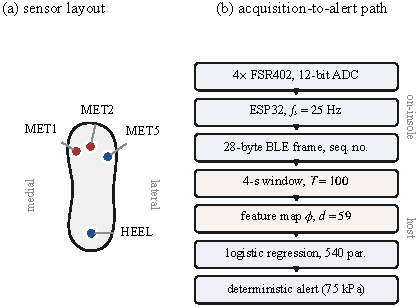
\includegraphics[width=\columnwidth]{figs/fig1_system.pdf}
\caption{(a) Canonical four-site layout for a right foot; the client strings
toes/ball/arch/heel are aliases of these sites only. Blue marks the sites whose
removal is expensive, red the two that are individually near free but jointly
load-bearing (Sec.~\ref{sec:game}). (b) Acquisition-to-alert path; the alert
stage is deterministic and no language model participates in scoring.}
\label{fig:system}
\end{figure}

\subsection{Transducer Model and Calibration}
\label{sec:cal}

Let $a_c[n]\in\{0,\dots,4095\}$ denote the ADC code on channel $c$ at sample
$n$ and $a_{0,c}$ an unloaded baseline. The shipped firmware applies the affine
placeholder $\hat p_c=(a_c-a_{0,c})\,p_{\max}/2^{12}$ with $p_{\max}=250$\,kPa,
which is a display convention rather than a fitted transducer curve. Because
the resistance of a force-sensitive polymer follows an approximate power law in
applied force, the divider output is linear in $\log F$ on a log--log scale, so
we invert the divider $R_c=R_f(4095/a_c-1)$ with $R_f=10\,\mathrm{k}\Omega$ and fit
\begin{equation}
\log_{10} \hat F_c = b_c \log_{10} R_c + \log_{10} k_c,
\qquad \hat p_c = \hat F_c / A_{\mathrm{eff}},
\label{eq:cal}
\end{equation}
obtaining $(k_c,b_c)=(1.74\times10^{5},-1.212)$,
$(1.06\times10^{5},-1.178)$,
$(3.16\times10^{5},-1.250)$ and
$(8.57\times10^{4},-1.174)$ at MET1, MET2, MET5 and the heel.
Differentiating \eqref{eq:cal} gives
\begin{equation}
\frac{\delta \hat F_c}{\hat F_c}
   = b_c\,\frac{\delta R_c}{R_c},
\label{eq:sens}
\end{equation}
so relative force error is amplified by $|b_c|\approx 1.2$ and diverges as
$a_c$ approaches the unloaded baseline, where $R_c$ becomes large; low-pressure
regions are therefore the least trustworthy part of the range, which is exactly
where the 30\,kPa contact threshold of Sec.~\ref{sec:feat} sits.

The four sites were bench-loaded across twelve commanded loads from 0 to
30\,N over five load--unload trials, giving 480 operator-attested ADC--force
pairs ($12\times5\times4$ sites $\times\,2$ directions). Reconstruction under
\eqref{eq:cal} gave mean absolute error (MAE) 1.69\,N, root-mean-square error
(RMSE) 2.95\,N and mean load--unload hysteresis 2.02\,N, with per-site MAE in
the range 1.44--2.16\,N.

\subsection{From Calibration Error to Classifier Faults}
\label{sec:budget}

Force errors acquire meaning only once expressed in the units the classifier
consumes. Taking the nominal 12.7\,mm active diameter of the FSR402 class,
$A_{\mathrm{eff}}=1.27$\,cm$^2$, so the MAE corresponds to roughly 13\,kPa, the
hysteresis to 16\,kPa and the RMSE to 23\,kPa. The perturbations that degrade
the classifier in Sec.~\ref{sec:robust}---12\,kPa of zero-mean noise and a
$+15$\,kPa constant offset---therefore sit \emph{inside} the transducer's own
error budget rather than outside it, as Fig.~\ref{fig:budget}(b) shows
directly.

This does not invalidate results obtained on a simulator whose pressures are
exact by construction, but it bounds what may be transferred from them. In
particular it demotes per-window baseline re-estimation and hysteresis
compensation from refinements to prerequisites: a device whose systematic error
is of the same order as the fault that destroys the model has no margin to
spend. Calibration error and classification accuracy remain distinct
quantities and are reported separately throughout.

\subsection{Windowing, Feature Map and Equivariance}
\label{sec:feat}

Analysis operates on a non-negative array
$P\in\mathbb{R}_{\ge0}^{T\times 8}$ with $T=100$: a fixed 4\,s window at
25\,Hz over sites $i\in\mathcal{S}=\{\mathrm{MET1},\mathrm{MET2},
\mathrm{MET5},\mathrm{HEEL}\}$ and feet $f\in\{L,R\}$, with no stride-cut
segmentation. The feature map $\phi:\mathbb{R}^{T\times8}\to\mathbb{R}^{59}$
computes, per site, the peak pressure $P^{\ast}_i=\max_t p_i(t)$, the mean
pressure, the coefficient of variation, the pressure--time integral
\begin{equation}
\mathrm{PTI}_i = \sum_{t} p_i(t)\,\Delta t, \qquad \Delta t = 1/f_s,
\label{eq:pti}
\end{equation}
threshold occupancies at a contact level $\tau_c=30$\,kPa and a high-pressure
level $\tau_h=200$\,kPa,
\begin{equation}
O_i(\tau) = \frac{1}{T}\sum_{t} \mathbf{1}\!\left[p_i(t)>\tau\right],
\label{eq:occ}
\end{equation}
and a bilateral asymmetry index
\begin{equation}
A_i = \bigl|P_i^{\ast L}-P_i^{\ast R}\bigr| \big/
      \max\!\left(\tfrac{1}{2}\bigl(P_i^{\ast L}+P_i^{\ast R}\bigr),\varepsilon\right),
\label{eq:asym}
\end{equation}
together with window-level cadence, stance ratio, anterior pressure share,
aggregate peak and total PTI: 59 named features in total.

Their behaviour under a constant offset is not uniform, and the difference
predicts the robustness results before any experiment is run. Write
$T_\delta p = p+\delta$. Then $P^{\ast}_i$ and the mean shift by $\delta$,
$\mathrm{PTI}_i$ shifts by $\delta T \Delta t$, and the asymmetry index
\eqref{eq:asym} is affected only through its denominator; all of these are
gently perturbed. The occupancies \eqref{eq:occ} are not, because
\begin{equation}
\frac{\partial}{\partial\delta}\,
\mathbb{E}\!\left[O_i(\tau)\bigm| T_\delta p_i\right]
   = f_{p_i}(\tau),
\label{eq:occsens}
\end{equation}
the probability density of $p_i$ evaluated at the threshold. A window whose
pressures cluster near $\tau_c$---which is the common case for a lightly loaded
site---therefore has its contact feature driven towards saturation by an offset
far smaller than the signal range, while a zero-mean perturbation of the same
magnitude leaves $\mathbb{E}[O_i]$ to first order unchanged. Equation
\eqref{eq:occsens} is the mechanism behind the gap between the noise and bias
rows of Table~\ref{tab:robust}.

\medskip
\noindent\textbf{Remark 1 (offset invariance).}\;
Let $Q_\alpha(\cdot)$ be the empirical $\alpha$-quantile of a window and define
$\tilde p_i = p_i - Q_{\alpha}(p_i)$ for a fixed low $\alpha$, e.g.\
$\alpha=0.05$. Quantiles are translation-equivariant,
$Q_\alpha(p+\delta)=Q_\alpha(p)+\delta$, so $\tilde p_i$ is invariant to any
constant offset, and hence so is every feature computed from $\tilde p_i$,
including \eqref{eq:occ}. Re-baselining per window therefore removes the
dominant failure mode of Sec.~\ref{sec:robust} at the cost of one order
statistic per site per window.

\medskip
\noindent The corresponding statement for a multiplicative gain error is
weaker, since normalising by an interquantile range would buy scale invariance
at the price of the absolute 75\,kPa alert operating point. The present release
implements neither correction; we report the consequence rather than patching
it after the fact. That 75\,kPa cut-off is itself an engineering operating
point on simulator labels, not a validated ulceration threshold.

% =====================================================================
\section{Evaluation Protocol}
\label{sec:proto}

\subsection{Data Sources}

Three sources are used and never mixed.
(a)~A synthetic four-FSR cohort (seed 67): 24 virtual subjects, 9
overload-pattern classes, 2592 windows at 25\,Hz with 3.5\,kPa Gaussian noise
and 3\% label flips; each virtual subject contributes 108 windows, i.e.\
7.2\,min of simulated wear, and every machine-learning number in this paper
comes from it.
(b)~The 480-row bench calibration table of Sec.~\ref{sec:cal}.
(c)~An independent archive of 15 healthy adults (7 female, 8 male; age 19--30
years) walking overground with a 32-cell instrumented insole synchronised to
optical motion capture \cite{zenodo2026}, of which 149 of 150 takes were
analysed; it serves only as sparse-versus-dense evidence.
No X-Step four-site walking sessions exist in this release ($N=0$), and no
clinical outcomes are available.

\subsection{Estimands}

Performance is not one quantity, and naming the target explicitly removes most
of the ambiguity that surrounds small-cohort wearable results. We distinguish
$R_{\mathrm{sub}}$, the expected macro-F1 on a window drawn from an
\emph{unseen} subject of the same generator; $R_{\mathrm{win}}$, the same for
an unseen window from a \emph{seen} subject; and $R_{\mathrm{hold}}$, equal in
target to $R_{\mathrm{sub}}$ but estimated on a single 25\% subject holdout and
therefore much higher in variance. $R_{\mathrm{sub}}$ is primary and is
estimated from pooled out-of-fold predictions under five-fold GroupKFold by
subject; pooling rather than averaging per-fold scores is necessary because
macro-F1 is not a mean of per-sample losses. Whenever subject identity carries
signal, $R_{\mathrm{win}}\ge R_{\mathrm{sub}}$, so the independent-window
control is optimistic by construction and the difference between the two is
interpretable in its own right: it is the price of transfer to a new wearer,
not merely a bookkeeping error. Session-grouped and leave-one-subject-out
splits are further controls, and automated leakage tests fail the build if
subject or session identifiers cross a forbidden partition.

\subsection{Statistical Inference}
\label{sec:stats}

Nine algorithms were fixed a priori---a peak-pressure threshold heuristic and a
majority dummy, logistic regression (the production head), decision trees,
ensembles and a multilayer perceptron. No hyperparameter search touched a test
partition, and standardisation sits inside the pipeline, fitted on training
folds only. Macro-F1 is the primary metric; accuracy, area under the receiver
operating characteristic curve (AUROC), Brier score and expected calibration
error (ECE) are secondary and uncorrected.

Uncertainty is the weak point of studies at this scale, so we state the
resampling unit explicitly. Windows within a subject are not independent, and a
percentile bootstrap over windows ignores that dependence. For a cluster size
$m=108$ and intra-cluster correlation $\rho$, the design effect
$\mathrm{DEFF}=1+(m-1)\rho$ equals 6.4 at $\rho=0.05$ and 22.4 at $\rho=0.2$,
reducing 2592 windows to an effective 408 or 116. The resampling unit is
therefore the subject, with $B=2000$ cluster bootstrap replicates; interval
half-widths shrink only as $O(n_{\mathrm{sub}}^{-1/2})$ with
$n_{\mathrm{sub}}=24$, which is the binding constraint on every comparison
below. The intervals printed in Table~\ref{tab:models} are window-level and
should be read as \emph{lower bounds} on interval width; under subject-cluster
resampling the production model gives 0.885 [0.861--0.907].

Model contrasts are paired on folds and tested with the same cluster bootstrap
applied to the difference, under Holm--Bonferroni control at family
$\alpha=0.05$ across the eight non-dummy comparisons \cite{holm1979}. Naive
resampled $t$-tests are avoided because their variance is underestimated when
training sets overlap across folds \cite{nadeau2003}. Claims of
\emph{equivalence} are tested rather than inferred from overlapping intervals,
using two one-sided tests (TOST) with a margin $\delta=0.02$ macro-F1 fixed in
advance at less than half the measured subject-transfer gap.

\subsection{Ablation and Fault Operators}
\label{sec:ops}

Let $M_A$ zero the channels of a site set $A\subseteq\mathcal{S}$ on both feet.
Two regimes must be distinguished, and conflating them is a common source of
overstatement. Evaluating a model trained on intact data at $\phi(M_A P)$
measures the \emph{fault response} of a deployed artefact; retraining under the
mask measures the \emph{information content} of the retained sites. We report
the retraining regime throughout, with the feature dimension held at 59 so that
model capacity is constant, and write $v(A)$ for the grouped macro-F1 obtained
with retained set $A$.

Packet loss is applied as an independent Bernoulli mask over frames with
dropped samples \emph{zeroed} rather than held. Zeroing is the pessimistic
reconstruction, since it injects spurious low-pressure samples that deflate
both $P^{\ast}_i$ and \eqref{eq:occ}; a zero-order hold with an explicit gap
flag, which the sequence counter already supports, cannot do worse under any
monotone reading of those two features. The reported degradation is therefore
an \emph{upper bound} on the loss a competent firmware implementation would
suffer, not an estimate of it. Additive noise and constant bias are applied in
pressure units before feature extraction; rate reduction is applied by
decimation, after which \eqref{eq:pti} is recomputed with the matching
$\Delta t$ so that PTI remains rate-invariant by construction.

Splits, seeds and model artefacts are versioned with the code, and the leakage
tests run in continuous integration, so the estimand definitions are enforced
mechanically rather than asserted.

% =====================================================================
\section{Results}

\subsection{Classifier Comparison and the Cost of the Split}
\label{sec:models}

Logistic regression achieved macro-F1 0.885 [0.873--0.894] on grouped
out-of-fold predictions, with accuracy 0.885, AUROC 0.979, Brier score 0.180
and ECE 0.031 (Table~\ref{tab:models}); the contrast against the majority dummy
survives Holm correction at $p=4\times10^{-3}$. Histogram gradient boosting
scored 0.885 [0.875--0.898]. Overlapping intervals do not establish
equivalence, so the pre-specified TOST at $\delta=0.02$ was applied and
returned equivalence (90\% CI $[-0.0197,0.0151]$ inside $\pm0.02$, $p=0.047$); logistic regression is retained on size and
latency grounds in either case, at 7.7\,kB and 0.07\,ms against 3.5\,MB and
13.1\,ms for a random forest that scored lower (0.837). The production head has
$59\times9+9=540$ parameters and costs 531 multiply--accumulate operations per
window, which is why the artefact is small enough to ship to a phone.

Replacing subject-grouped with independent-window splitting raised the same
pipeline to 0.931. Under the framing of Sec.~\ref{sec:proto} the resulting
0.046 is an estimate of $R_{\mathrm{win}}-R_{\mathrm{sub}}$, and it is
indistinguishable in magnitude from the entire 0.048 spread between the best
and the worst trained classifier in the table. At this cohort size, evaluation
design is not a second-order concern relative to model choice.

\begin{table}[!t]
\caption{Classifier comparison under five-fold GroupKFold by virtual subject.
Split-protocol controls for logistic regression: session-grouped 0.880,
leave-one-subject-out 0.885. Brackets are window-level bootstrap 95\%
intervals and understate width (Sec.~\ref{sec:stats}).}
\label{tab:models}
\centering
\renewcommand{\arraystretch}{1.1}
\setlength{\tabcolsep}{3pt}
\scriptsize
\begin{tabular}{@{}llrrr@{}}
\toprule
Model & Macro-F1 [95\% CI] & Acc. & kB & ms \\
\midrule
Majority dummy           & 0.040 [0.036--0.043] & 0.111 & --     & --    \\
Threshold heuristic      & 0.480 [0.460--0.493] & 0.497 & 2.1    & 0.01  \\
Random forest            & 0.837 [0.824--0.851] & 0.834 & 3547.5 & 13.12 \\
Hist.\ grad.\ boosting   & 0.885 [0.875--0.898] & 0.885 & --     & --    \\
Logistic regr.\ (prod.)  & 0.885 [0.873--0.894] & 0.885 & 7.7    & 0.07  \\
IID windows (control)    & 0.931 [0.921--0.941] & 0.930 & --     & --    \\
\bottomrule
\end{tabular}
\end{table}

\subsection{How Much Label Information Four Sites Retain}
\label{sec:fano}

Macro-F1 is metric-specific and hard to compare across layouts of different
difficulty. Fano's inequality converts it into a scale that is not
\cite{cover2006}. For a balanced $K$-class problem with label $Y$, prediction
$\hat Y$ and error rate $P_e$,
\begin{equation}
H(Y\mid\hat Y)\;\le\;H_b(P_e)+P_e\log_2(K-1),
\label{eq:fano}
\end{equation}
with $H_b$ the binary entropy, so that by the data-processing inequality the
mutual information between the window and the label obeys
\begin{equation}
I(Y;X)\;\ge\;I(Y;\hat Y)\;\ge\;H(Y)-H_b(P_e)-P_e\log_2(K-1).
\label{eq:fanoI}
\end{equation}
Here $K=9$ and $H(Y)=\log_2 9 = 3.170$ bits. Applying \eqref{eq:fanoI} to the
production model gives $I\ge 2.310$ bits, so a 4\,s window from four sparse
sites retains at least 72.9\% of the label entropy of this generator. The bound
is a genuine lower bound and is tight at chance: the majority dummy, at
accuracy $1/9$, returns exactly 0.000 bits, which is a useful validity check on
the arithmetic.

Table~\ref{tab:fano} applies the same computation to every reported layout.
The transformation is strongly concave near the top of the range, which is why
layouts that look close on the F1 scale separate more slowly in bits and
layouts that look far apart compress: dropping MET5 costs 0.214 macro-F1 but
0.979 bits, while dropping MET1 costs 0.002 macro-F1 and 0.014 bits.

\begin{table}[!t]
\caption{Label information retained by each layout, from Fano's inequality
\eqref{eq:fanoI} with $K=9$, $H(Y)=3.170$ bits. $P_e$ is one minus grouped
out-of-fold accuracy (not macro-F1). Dummy accuracy 0.111 matches $1/9$ to three
decimals and returns 0.000 bits. All entries are lower bounds.}
\label{tab:fano}
\centering
\renewcommand{\arraystretch}{1.1}
\setlength{\tabcolsep}{4pt}
\scriptsize
\begin{tabular}{@{}lrrrr@{}}
\toprule
Retained layout & Macro-F1 & Acc. & $I\ge$ (bits) & \% of $H(Y)$ \\
\midrule
All four sites        & 0.885 & 0.885 & 2.310 & 72.9 \\
Drop MET1             & 0.883 & 0.883 & 2.297 & 72.4 \\
Drop MET2             & 0.874 & 0.875 & 2.254 & 71.1 \\
Drop MET5             & 0.671 & 0.686 & 1.332 & 42.0 \\
Drop HEEL             & 0.657 & 0.669 & 1.259 & 39.7 \\
MET2$+$HEEL (best pair) & 0.686 & 0.695 & 1.369 & 43.2 \\
MET1$+$MET2 only      & 0.435 & 0.459 & 0.553 & 17.4 \\
Best single site      & 0.420 & 0.449 & 0.524 & 16.5 \\
Majority dummy        & 0.040 & 0.111 & 0.000 & \phantom{0}0.0 \\
\bottomrule
\end{tabular}
\end{table}

\subsection{Layout Value as a Cooperative Game}
\label{sec:game}

Removing MET1 cost 0.002 macro-F1 and MET2 0.011, whereas removing MET5 cost
0.214 (to 0.671) and the heel 0.228 (to 0.657). Read as a ranking, this invites
the conclusion that MET1 is disposable. The cooperative-game reading forbids
it. Taking the dummy as the empty layout, the total attainable value is
$v(\mathcal{S})-v(\emptyset)=0.845$, whereas the four marginal contributions to
the grand coalition sum to only 0.455: marginals recover 54\% of the value, so
single-site attributions are not additive and must not be summed. Shapley values
over the 16-subset lattice are 0.152, 0.158, 0.254 and 0.280 for MET1, MET2,
MET5 and HEEL; they sum to the attainable 0.845 and assign 63\% of the credit to
MET5 and the heel. The interaction structure is already visible without them.
Define the second-order interaction
\begin{equation}
I(i,j)=\Delta_{ij}-\Delta_i-\Delta_j,\qquad
\Delta_A = v(\mathcal{S})-v(\mathcal{S}\setminus A).
\label{eq:inter}
\end{equation}
For MET5 and HEEL, the layout retaining only MET1$+$MET2 scored 0.435, giving
$\Delta_{ij}=0.450$ against $\Delta_i+\Delta_j=0.442$ and hence
$I=+0.008$: the two carry almost perfectly separate information. For MET1 and
MET2 the complementary two-site layout is MET5$+$HEEL (macro-F1 0.649), not the
best two-site pair MET2$+$HEEL (0.686), giving $\Delta_{ij}=0.236$ against a
summed 0.013 and $I=+0.223$, an interaction an order of magnitude larger than
either marginal. The forefoot sites are individually near free precisely because
they substitute for each other, and dropping both is not free at all.

Repeating the computation in bits sharpens the picture and corrects part of it.
On the information scale of Table~\ref{tab:fano} the four marginal
contributions sum to 2.100 bits against a total attainable 2.310, recovering
91\% rather than 54\%. Most of the apparent redundancy is therefore an
artefact of the concave map from information to macro-F1 rather than a property
of the sensor set: measured in bits, the four sites are close to additive. What
survives the change of scale is the interaction structure. MET1 and MET2 remain
strongly superadditive ($I=+1.001$ bits, from $\Delta_{ij}=1.071$ against a
summed 0.070), while MET5 and HEEL turn mildly subadditive ($I=-0.272$ bits),
indicating a modest overlap between rearfoot and lateral-forefoot information
that the F1 scale had hidden.

Every single-site layout collapsed to 0.39--0.42 macro-F1, and the
forefoot-only pair (0.435) is worse than any pair retaining a rear or lateral
channel, so anatomical coverage dominates sensor count. We retain MET1 as a
frequently reported clinical ulceration site \cite{armstrong2017,fernando2014}
at the cost of one ADC channel; Fig.~\ref{fig:layout} summarises both scales.

\begin{figure}[!t]
\centering
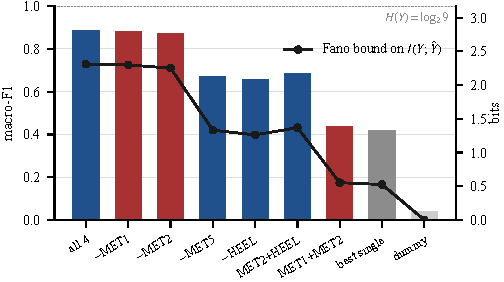
\includegraphics[width=\columnwidth]{figs/fig2_layout.pdf}
\caption{Layout value on the macro-F1 scale (bars) and the Fano information
scale (line, right axis). Red bars mark the two sites that are individually
near free but jointly load-bearing. The dashed line is the label entropy
$H(Y)=\log_2 9$; the dummy sits at exactly zero bits.}
\label{fig:layout}
\end{figure}

\subsection{Robustness, Alert Thresholds and Deployment}
\label{sec:robust}

Robustness uses a grouped 25\% subject holdout estimating $R_{\mathrm{hold}}$
with clean baseline 0.847. This is a different estimand from the out-of-fold
0.885 and the two should not be differenced (Table~\ref{tab:robust},
Fig.~\ref{fig:budget}). Degradation is graded for faults produced by the radio
link and abrupt for faults produced by the transducer: a dead heel channel and
a $+15$\,kPa offset each destroy the model, the latter by the
occupancy-saturation mechanism derived in \eqref{eq:occsens}, which Remark~1
shows is removable. Halving the effective rate to 12.5\,Hz was nearly free
(0.843) whereas 6.25\,Hz was costly (0.714), which implicates peak estimation
rather than the rate-invariant PTI: a 0.6\,s stance phase receives roughly
eight samples at 12.5\,Hz but fewer than four at 6.25\,Hz, making $P^{\ast}_i$
biased low by an amount that grows as the peak narrows.

Sweeping the alert cut-off gave sensitivity/specificity 0.844/0.316 at
40\,kPa, 0.681/0.933 at 55\,kPa and 0.427/0.986 at 75\,kPa: the shipped default
is deliberately specificity-weighted, a design choice about alert fatigue and
not a screening-sensitivity claim. Host-side, feature extraction averaged
0.16\,ms and inference 0.07\,ms for a combined 0.23\,ms path (P95 0.31\,ms,
$n=200$), a duty cycle of 0.6\% against the 40\,ms sample period. BLE airtime,
over-the-air error rate and battery life were not measured and are not
estimated here.

\begin{table}[!t]
\caption{Robustness and sampling-rate operating points on a grouped 25\%
subject holdout. Packet loss is simulated by zeroing time samples and is an
upper bound on degradation rather than an over-the-air measurement
(Sec.~\ref{sec:ops}).}
\label{tab:robust}
\centering
\renewcommand{\arraystretch}{1.1}
\setlength{\tabcolsep}{4pt}
\scriptsize
\begin{tabular}{@{}llrrr@{}}
\toprule
Perturbation & Severity & Perturbed & $\Delta$ & Rel. \\
\midrule
Gaussian noise      & 12\,kPa SD          & 0.641 & $-0.206$ & $-24\%$   \\
Dropped packets     & 30\%                & 0.631 & $-0.216$ & $-26\%$   \\
Missing channel     & HEEL $=0$           & 0.218 & $-0.629$ & $-74\%$   \\
Constant bias       & $+15$\,kPa          & 0.181 & $-0.666$ & $-79\%$   \\
Rate reduction      & 50\% (12.5\,Hz)     & 0.843 & $-0.004$ & $-0.5\%$  \\
\bottomrule
\end{tabular}
\end{table}

\begin{figure}[!t]
\centering
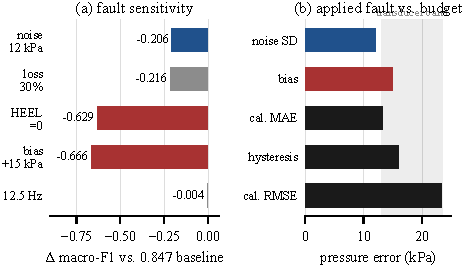
\includegraphics[width=\columnwidth]{figs/fig3_budget.pdf}
\caption{(a) Fault sensitivity against the 0.847 clean holdout baseline.
(b) The magnitude of the applied faults compared with the transducer's own
pressure-equivalent error budget from Sec.~\ref{sec:budget}; the shaded band
spans calibration MAE to RMSE. The two faults that were injected lie inside the
band, which limits what the robustness curves can be transferred to.}
\label{fig:budget}
\end{figure}

\subsection{Sparse Versus Dense Sites in Human Walking}
\label{sec:dense}

Because no X-Step walking data exist, the sparse-sampling assumption was probed
on the 32-cell archive by comparing single anatomical cells against the maximum
of the corresponding dense cluster (298 foot-takes). Median time-series
correlation was 0.986 at MET2, 0.885 at the heel, 0.879 at MET1 and 0.717 at
MET5. Pearson correlation is invariant under affine rescaling, so these values
certify waveform \emph{shape} and are silent on magnitude; the peak-to-peak
correlations of 0.43--0.74 are the relevant statistic, and proper limits of
agreement \cite{bland1986} are unavailable across hardware reporting different
native units without a cross-calibration we do not have.

A four-site reconstruction of the centre of pressure,
$\hat{c}(t)=\sum_i \mathbf{x}_i p_i(t)/\sum_i p_i(t)$, tracked the
anteroposterior component (median $r=0.805$) but not the mediolateral one
($r=0.005$). This is expected geometrically as well as empirically. Since
$\hat c(t)$ is a convex combination of the site coordinates,
$\hat c(t)\in\mathrm{conv}\{\mathbf{x}_i\}$ for all $t$, so for any reference
point $\bar{\mathbf{x}}$ the reconstructed excursion satisfies
$\|\hat c(t)-\bar{\mathbf{x}}\|\le\max_i\|\mathbf{x}_i-\bar{\mathbf{x}}\|$: a
four-point measure systematically contracts the true excursion, and with no
medial--lateral pair in the midfoot the mediolateral coordinate is nearly fixed
by the site geometry. None of these values enter the classification tables.

% =====================================================================
\section{Discussion and Threats to Validity}

Three evidence levels should be kept apart. Level~A is physical engineering
evidence: calibration, timing, packet accounting, latency. Level~B is
algorithmic evidence on a stated dataset. Level~C is clinical evidence:
incident ulceration, prevented events, decision impact. This paper contributes
Level~A and Level~B, plus a Level~A/B sparse-versus-dense comparison on
different hardware. It contributes nothing at Level~C: a grouped macro-F1 of
0.885, or 2.31 bits, is a statement about a generator and not about a patient.

The dominant threat is to \emph{construct} validity. Simulator zone labels are
a deterministic function of gait class, and peak-only features reached 0.886
against 0.885 for the full 59-dimensional vector, so the generator is largely
peak-separable and the problem posed here is narrower than the one a wearer
presents; the 2.31-bit figure is a property of that generator's label entropy,
not of human gait. \emph{Internal} validity is protected by grouped splitting
and automated leakage tests, but the robustness grid, the ablation lattice and
the threshold sweep were all computed after the production head was frozen,
which is the correct order yet still selects an operating point on the same
generator it is evaluated on. \emph{Statistical-conclusion} validity is limited
by 24 clusters: the cluster bootstrap of Sec.~\ref{sec:stats} has little
resolution below the $\delta=0.02$ margin, which is precisely why equivalence
is tested rather than asserted, and why the Fano column of
Table~\ref{tab:fano} is reported as a bound rather than an estimate.
\emph{External} validity is weakest: four resistive sensors cannot reconstruct
shear or a full pressure map, drift and creep are not bench-quantified, radio
airtime and battery life are unmeasured so no wear-time claim is made, and
test--retest reliability characterises the generator only. An unpaired
ulcer-image classifier in the repository is excluded, since pairing it with
insole data would imply a fusion result we cannot support, and no ethics
approval accompanies the reused archive.

Three findings nevertheless generalise as design guidance. Evaluation design
dominates apparent performance at this scale. Sparse layouts fail
asymmetrically, so sequence-gap accounting and per-channel plausibility checks
matter more than a smoothly degrading score, which will silently mislead when
an electrode lifts. And redundancy, not rank, is the right frame for site
selection: the site whose removal is cheapest may be the one whose partner is
doing its work, a conclusion that only becomes visible once layouts are scored
as coalitions rather than ranked individually.

% =====================================================================
\section{Conclusion}

X-Step specifies a four-site plantar-pressure insole with a documented 28-byte
BLE contract, operator-attested transducer calibration placed in an explicit
error budget, a leakage-controlled modelling stack with pre-specified estimands
and subject-cluster inference, and ablation, robustness and host-latency
operating curves. Under subject-grouped evaluation the production head reaches
macro-F1 0.885---at least 2.31 of 3.17 bits of label information---at 7.7\,kB
and 0.23\,ms of host path. It degrades gracefully under noise, bounded packet
loss and halved sampling rate, and fails outright under channel loss or
constant bias, the latter predictable from the threshold features themselves
and removable by per-window re-baselining. Scored as a cooperative game, the
four sites are nearly additive in bits but strongly interacting in pairs, so
MET5 and HEEL carry separate information while the forefoot pair is internally
redundant and jointly load-bearing. Offset-equivariant features, measured radio
and power figures, bench characterisation of drift over wear cycles, and a
prospective walking study under ethics approval are the bridge to any
patient-facing statement.

% =====================================================================
\begin{thebibliography}{99}
\footnotesize
\setlength{\itemsep}{0pt plus 0.2pt}

\bibitem{armstrong2017}
D.~G. Armstrong, A.~J.~M. Boulton, and S.~A. Bus, ``Diabetic foot ulcers and
their recurrence,'' \emph{N. Engl. J. Med.}, vol.~376, no.~24, pp.
2367--2375, 2017.

\bibitem{fernando2014}
M.~E. Fernando \emph{et~al.}, ``Plantar pressure in diabetic peripheral
neuropathy patients with active foot ulceration, previous ulceration and no
history of ulceration: a meta-analysis of observational studies,''
\emph{PLoS ONE}, vol.~9, no.~6, p. e99050, 2014.

\bibitem{iwgdf2023}
N.~C. Schaper \emph{et~al.}, ``Practical guidelines on the prevention and
management of diabetes-related foot disease (IWGDF 2023 update),''
\emph{Diabetes Metab. Res. Rev.}, vol.~40, p. e3657, 2024.

\bibitem{bus2016}
S.~A. Bus \emph{et~al.}, ``Footwear and offloading interventions to prevent and
heal foot ulcers and reduce plantar pressure in patients with diabetes: a
systematic review,'' \emph{Diabetes Metab. Res. Rev.}, vol.~32, no.~S1, pp.
99--118, 2016.

\bibitem{cavanagh2010}
P.~R. Cavanagh and S.~A. Bus, ``Off-loading the diabetic foot for ulcer
prevention and healing,'' \emph{J. Vasc. Surg.}, vol.~52, no.~3S, pp.
37S--43S, 2010.

\bibitem{razak2012}
A.~H. Abdul Razak, A.~Zayegh, R.~K. Begg, and Y.~Wahab, ``Foot plantar pressure
measurement system: a review,'' \emph{Sensors}, vol.~12, no.~7, pp.
9884--9912, 2012.

\bibitem{hegde2016}
N.~Hegde, M.~Bries, and E.~Sazonov, ``A comparative review of footwear-based
wearable systems,'' \emph{Electronics}, vol.~5, no.~3, p.~48, 2016.

\bibitem{hegde2014}
N.~Hegde and E.~Sazonov, ``SmartStep: a fully integrated, low-power insole
monitor,'' \emph{Electronics}, vol.~3, no.~2, pp. 381--397, 2014.

\bibitem{armstrong2007}
D.~G. Armstrong, K.~Holtz-Neiderer, C.~Wendel \emph{et~al.}, ``Skin temperature
monitoring reduces the risk for diabetic foot ulceration in high-risk
patients,'' \emph{Am. J. Med.}, vol.~120, no.~12, pp. 1042--1046, 2007.

\bibitem{holm1979}
S.~Holm, ``A simple sequentially rejective multiple test procedure,''
\emph{Scand. J. Stat.}, vol.~6, no.~2, pp. 65--70, 1979.

\bibitem{nadeau2003}
C.~Nadeau and Y.~Bengio, ``Inference for the generalization error,''
\emph{Mach. Learn.}, vol.~52, no.~3, pp. 239--281, 2003.

\bibitem{bland1986}
J.~M. Bland and D.~G. Altman, ``Statistical methods for assessing agreement
between two methods of clinical measurement,'' \emph{Lancet}, vol.~327, no.
8476, pp. 307--310, 1986.

\bibitem{cover2006}
T.~M. Cover and J.~A. Thomas, \emph{Elements of Information Theory}, 2nd~ed.
Hoboken, NJ, USA: Wiley, 2006.

\bibitem{zenodo2026}
``Multimodal gait dataset: synchronized sensorized-insole (pressure and
inertial) and optical motion-capture recordings,'' Zenodo, 2026. doi:
10.5281/zenodo.20156243.

\end{thebibliography}

\end{document}
